\section{Experiments And Results}
\label{sec:evaluation}
As described in section \ref{sec:visual-aspects} applying the deep dream works by selecting layers and neurons that will enhance recognized features within the image.
In order to select good layers for visualization, we apply each layer to a reference image and then handpick the layers that offer interesting features. The result of that can be seen in section \ref{sec:withoutguide}.
By selecting only one layer we do not limit ourselves to specific neuron within the layer. Combining multiple layers features with each other is also not done through that technique. That is why, in section \ref{sec:withguide}, we will use the \emph{guided dreaming} presented in section \ref{guided-dreaming} to select multiple layers and neurons via a guide image.
To apply the \emph{dream} we use a slightly modified version of the original google deep dream code for the neural network framework caffe\cite{googledeepdream}.

\subsection{Performance Considerations}
The runtime of deep dreaming depends mostly on the size of the input image.
Using an image of $\approx$600x430 pixels it can already take around 45 minutes to apply and uses up to 14gb of RAM.
We also introduced the bilateral filter which we will try to apply at every step. This will also heavily slow down the runtime because the application of the filter takes a few seconds and is applied at every step of modification.
%TODO bilateral vorher iwo mal erwähnen in intro
\subsection{Without Guide Image}
\label{sec:withoutguide}
The analyzed model contains 50 layers, so we will not be showing each one, but rather a selection of the ones we deemed most interesting.
Within the layers many things from varying colors, basic features to parts of distinct objects.
Looking at (layer 15/18 + 13/14) one can see that the recognizable features within a layer are definitely not limited to a particular one and also includes transitions(layer 13/14). These transitions can either distinguish pixelated regions to very sharp ones. But it can also result in a transition from smooth curves to very straight lines (layer16/18).
Going further up in the layers we found one layer of particular interest, depicted in figure \ref{fig:layer-snake}. It visualizes four distinct things at once which makes it unique. The scales of a snake with it's head in the lower left part of the image Also to the right of the very left house is a small part of a snakes face visible that seems to contain an eye and two teeth. Apart from these two already distinctive objects the center seems to contain the right part of a dog face and above that the sky looks more like dog fur than snake scales. 

\begin{figure}[H]
	\centering
	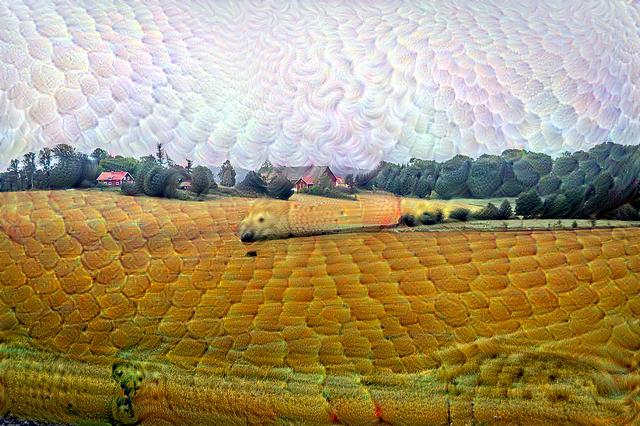
\includegraphics[width=0.5\linewidth]{img/alpsted-landscape_res4f_branch2a.jpg}
	\caption{Layer 41 \emph{res4f\_branch2a}. Seems like snake scales with a snake head in the lower left.}
	\label{fig:layer-snake}
\end{figure}


%TODO: beispiel hohe stepsize => visualisierung von haus o.a.
\subsection{With Guide Image}
\label{sec:withguide}
